\subsection{Tracking system}

%\subsubsection{The vertex locator}

%\subsubsection{Tracking detectors}


The tracking system of \lhcb consists of a VErtex LOcator(\velo), four tracking stations and a warm dipole magnet.
The \velo is positioned around the interaction points, and 
there is one tracking station after the \velo and before the magnet, the Tracker Turenscis (\ttracker).
Downstream of the magnet, there are three tracking stations, made from an Inner Tracker (\intr) and an Outer Tracker (\ot).

The \velo provides precise measurements of tracks that originate close to the vertices of the proton-proton interactions.
This allows the primary vertices, where the $pp$ interaction takes place, to be distinguished from the 
secondary and tertiary vertices which are distinct properties of \B decays.
The \velo is a silicon tracker with modules that provide radial ($r$) and polar ($\phi$) information for tracks. 
The \velo has a geometrical acceptance from $1.6<\eta<4.9$.
The arrangement of the sensors into the $r-\phi$ geometry was chosen in order to permit fast reconstruction of
the tracks in the trigger, as described in Section~\ref{sec:lhcb:trig}.
The geometry of the \velo sensors is illustrated in Fig.~\ref{fig:lhcb:velo}.
\begin{figure}[tbp]
\centering
\subfigure[]{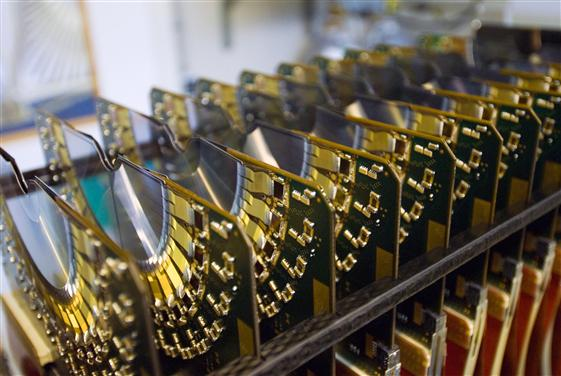
\includegraphics[width=0.48\columnwidth]{chapter3/figs/velopic.jpg}}
\subfigure[]{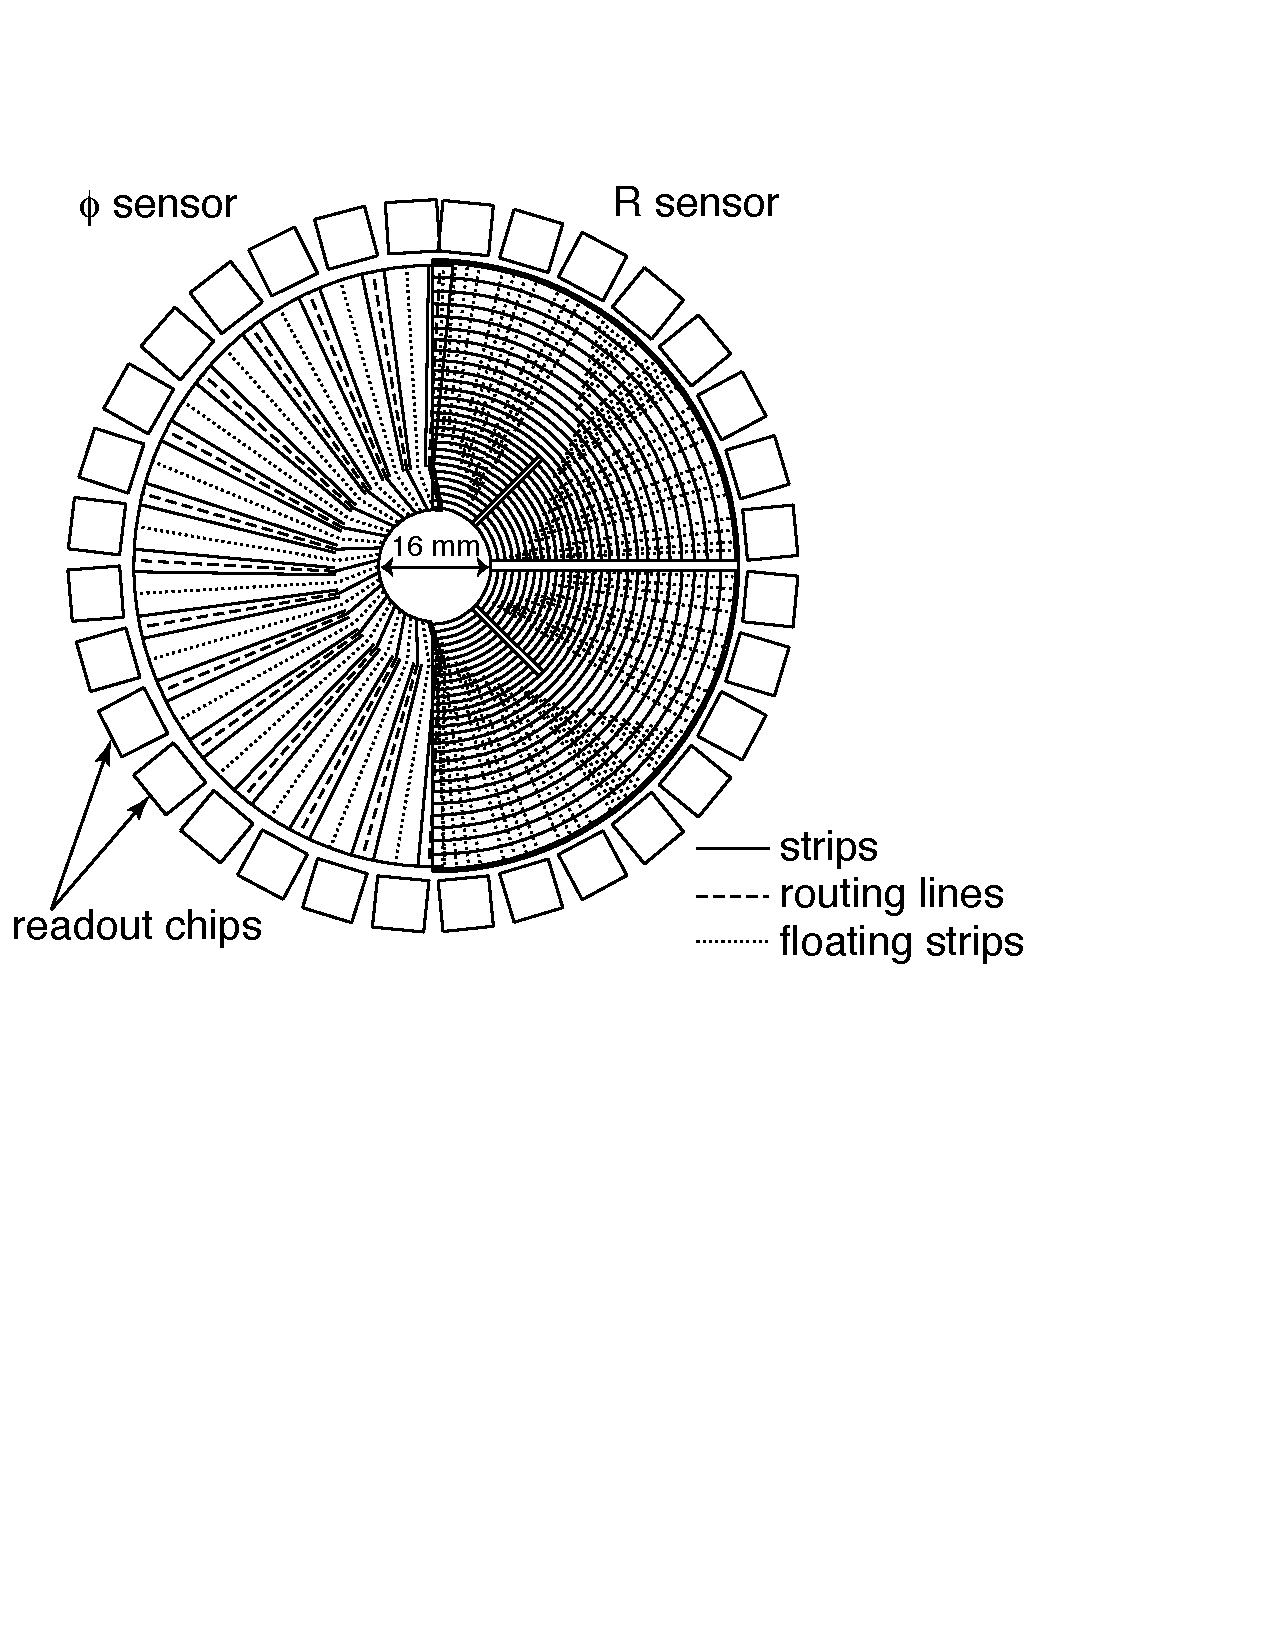
\includegraphics[width=0.48\columnwidth]{chapter3/figs/velodisc.pdf}}
\caption[The \velo.]{(a) One half of the \velo showing the hemispherical silicon detectors~\cite{Maximilien:1024838}
(b) The  geometry of the \velo illustrating the $r-\phi$ arrangement of the silicon sensors.~\label{fig:lhcb:velo}}
\end{figure}
The \velo was constructed in  two halves so that the detector can be moved closer to the interaction point  from each side
 once the beams are in a stable configuration. 
%This allows the \velo to be moved away from the beams to protect the sensors from damage when they are being injected to the \lhc and being accelerated. 
%In addition to the mechanical protection, there is both aluminium foil between the sensors and the beam to protect the sensors 
%from electrical currents induced by proximity to the beams and the \velo is also operated at -5 degrees Centigrade.
%\begin{figure}[tbp]
%\centering
%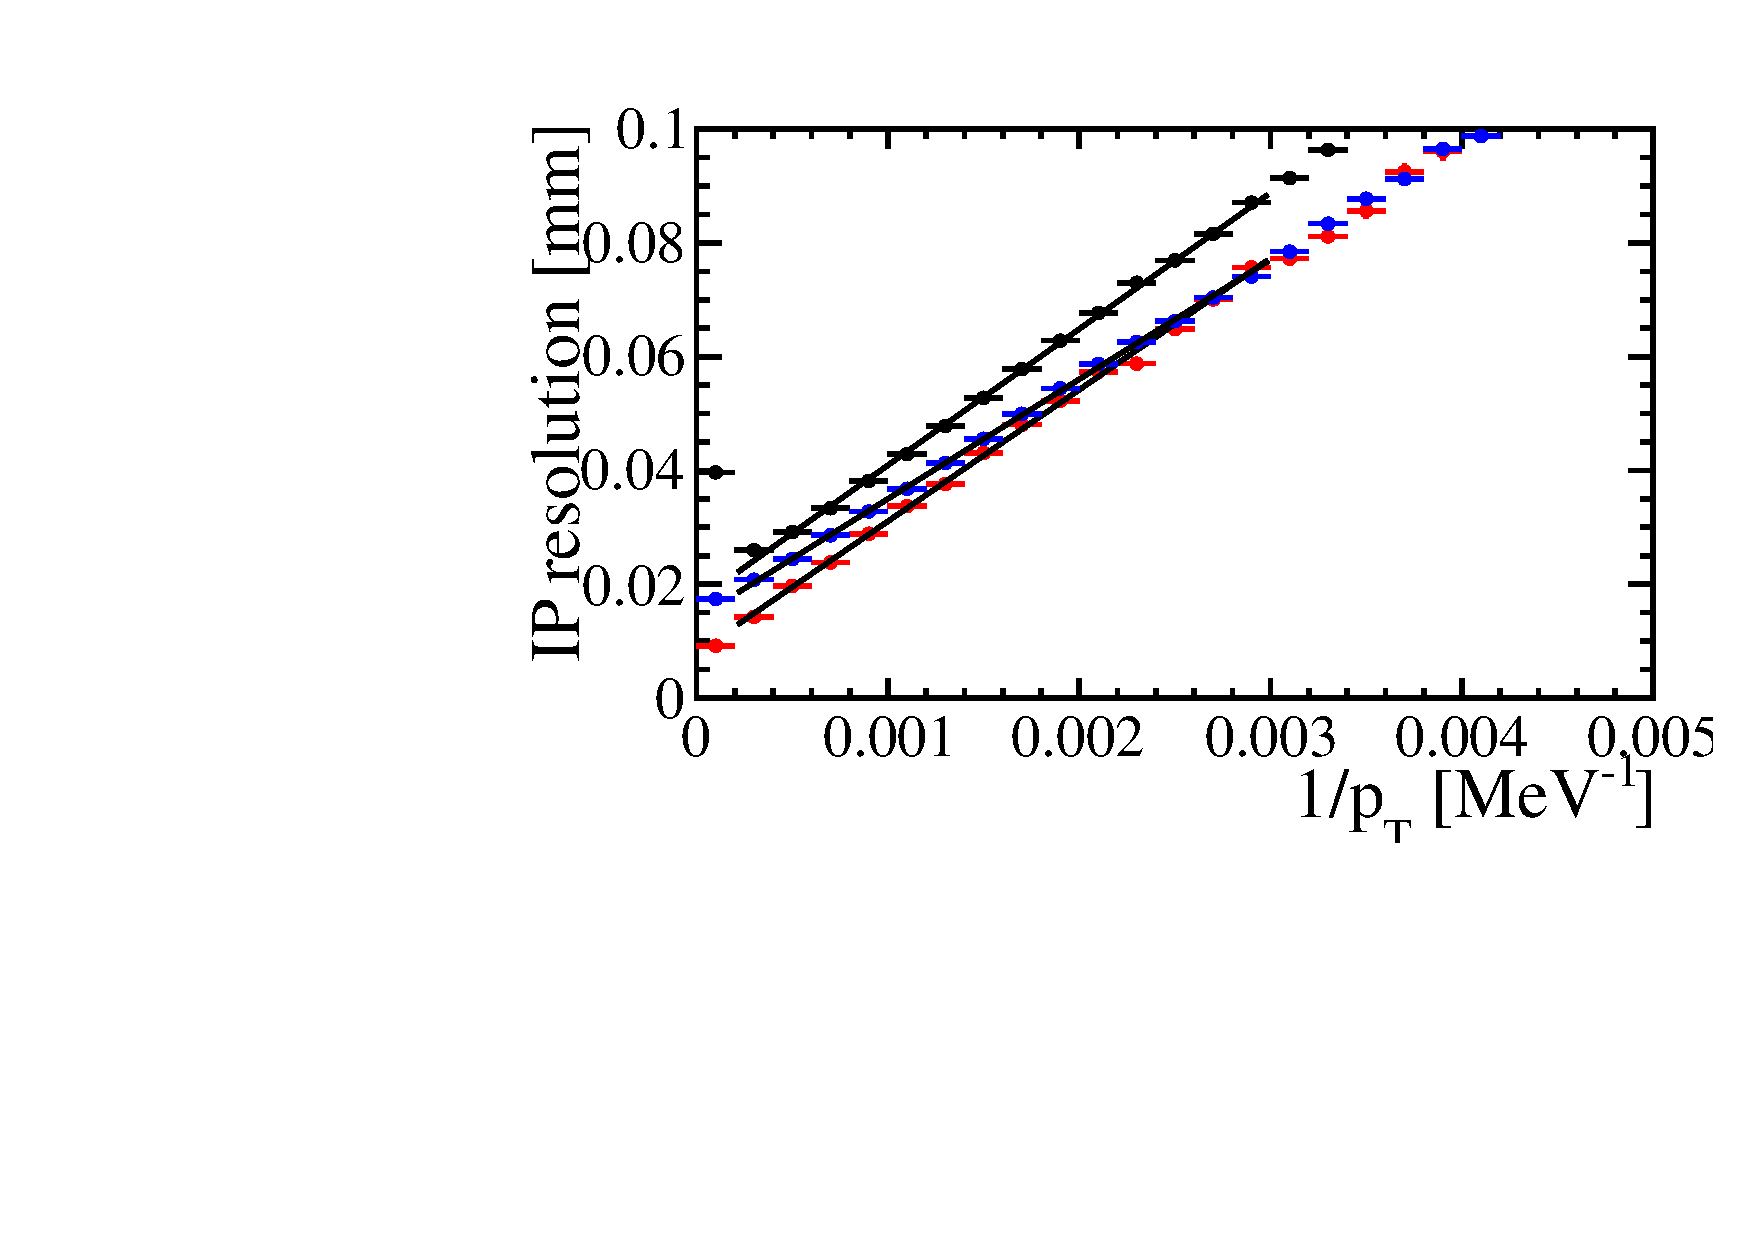
\includegraphics[width=0.48\columnwidth]{chapter3/figs/ipres_data_mc10_mc11.pdf}
%\caption{The IP resolution of data, MC10 and MC11 . [REF]~\label{fig:lhcb:ipres}}
%\end{figure}

The \ttracker is a 150\cm by 130\cm silicon strip detector which covers the full acceptance of the detector.
The \intr is placed in the region close to the beam pipe which has a very high occupancy of tracks, 
as measured in~\cite{LHCb-PAPER-2011-011},
and is made from the same silicon strips as the \ttracker, covering a total area of 120 by 40\cm.
The \ot encompasses the regions with lower particle density out to 250\cm in the vertical place and 300\cm in the horizontal plane.
Each of the \ot detectors is made out of straw tubes containing a mixture of argon and \cotwo, 
which were chosen to give a fast read-out time of less than 50\ns and to have a drift co-ordinate resolution of 200\mum.

The \lhcb magnet is a warm dipole magnet with an integrated field strength of 4 Tm. 
The magnet covers the full \lhcb acceptance with an area of 250\cm by 300 \cm.
The magnet was designed to minimise the magnetic field in the \rich detectors and to also maximise the field strength between
the tracking stations. 
This is because the photon detectors used to detect Cherenkov radiation in the \rich detectors are highly sensitive to stray magnetic fields.
The bending plane of the magnet is in the horizontal plane and data is taken with both magnet polarities in roughly equal amounts.

%The geometry of the tracking system leads to three different types of tracks that can be reconstructed in \lhcb.
%The most common category is 'Long' tracks, which pass through all the tracking stations.
%There are two sets tracks which do not pass through the full detector, these are 'Upstream' and 'Downstream'.
%The upstream tracks only pass through the \velo and the \ttracker and are swept out 
% of acceptance by the magnetic field. 
%The downstream tracks come from long-lived particles which decay after passing through the \velo such \KS and \L particles.
%These then pass through the \ttracker and the downstream tracking stations.
%The different track types along with the magnetic field strength are shown in Fig.~\ref{fig:lhcb:tracking}.
%\begin{figure}[tbp]
%\centering
%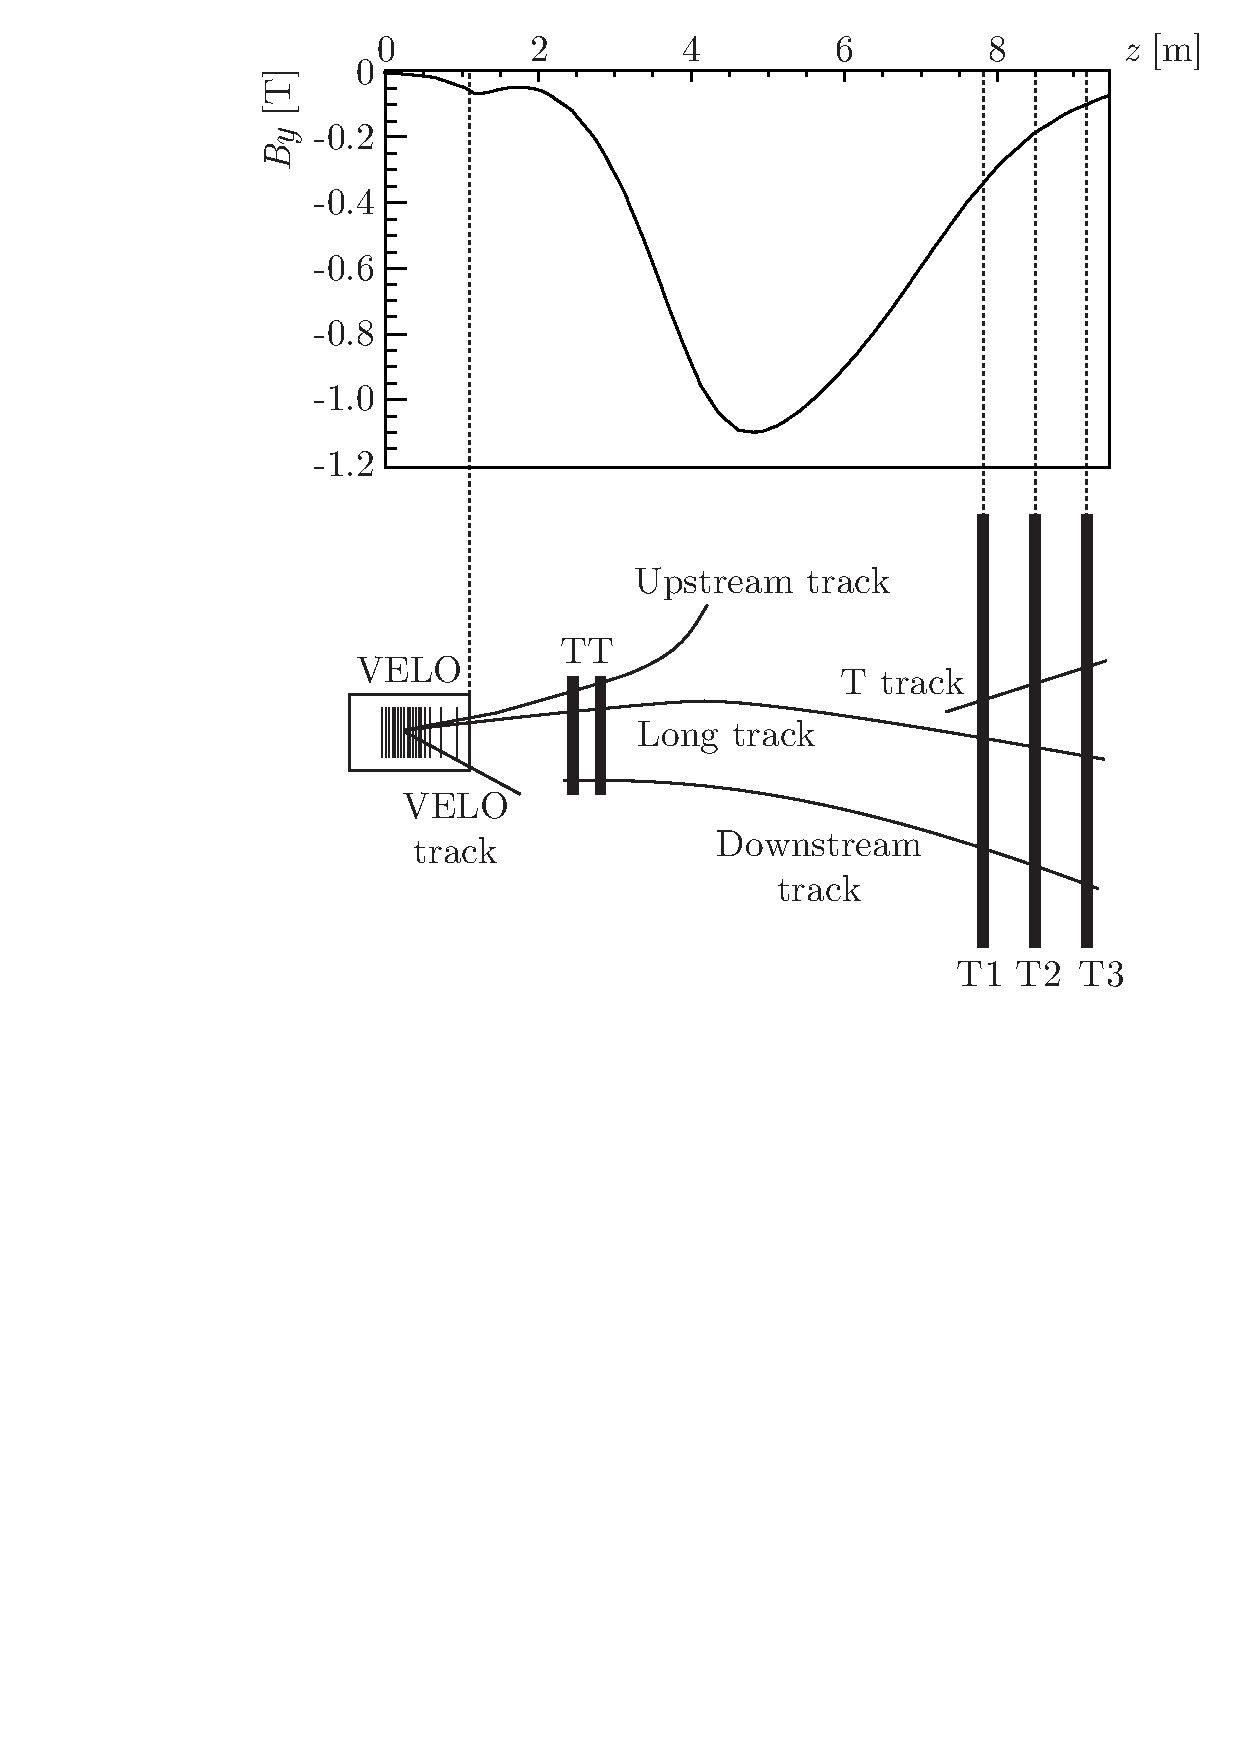
\includegraphics[width=0.48\columnwidth]{chapter3/figs/tracktypes.pdf}
%\caption{The three different types of tracks reconstructed using the \lhcb tracking system and the magnetic field strength throughout the detector.
% Long tracks and upstream tracks originate inside the \velo and pass through the \ttracker. Upstream tracks are swept out of the detector acceptance by the magnet whilst
%Downstream tracks originate from long-lived particles and have their first hits in the \ttracker. ~\cite{Alves:2008zz}.~\label{fig:lhcb:tracking}}
%\end{figure}

The performance of the track reconstruction in \lhcb can be evaluated by measuring the tracking efficiency
using the `tag-and-probe' method~\cite{Jaeger:1402577} .
The `tag-and-probe' method takes a fully reconstructed two-body decay, such as  \decay{\Z}{\mumu} or \decay{\jpsi}{\mumu}, 
 and looks for the probability that one of the daughters is found ( the `probe') given the reconstruction of the other daughter (the `tag').
The tracking efficiency overall is around 96\% for the data taken in 2011 and is flat in $\eta$ and in the momentum range from $10$ to $200\gev$.

\subsection{Particle identification }

\subsubsection{ Charged hadron identification }

The identification of charged hadrons is provided by two Ring Imaging Cherenkov (\rich) detectors which 
 provide particle identification over a large momentum range from 2 to 100 \gevc.
The \rich detectors distinguish pions, kaons and protons through measurements of the Cherenkov angle of particles
which pass through the detector.
These particles are travelling faster than the phase velocity of light in the detector gas and therefore emit Cherenkov radiation
 in a cone around the track.
The opening angle of this cone ($\theta_c$) is related to the velocity of the particle through $\theta_c = (n\beta)^{-1}$ 
where $n$ is the refractive index of the material.
A measurement of $\theta_c$ combined with  momentum information
from the tracking system provides a measurement of the mass of the particle.
This differentiation of charged particles allows dramatic reductions in the 
the level of combinatorial background for \B decays which have several hadrons in the final state.
For \BdToKstll, this is of critical importance in  the separation of pions and kaons.

The optical system of the \rich detectors consists of two components, a tilted spherical mirror 
to focus the Cherenkov light  and 
a second flat mirror to guide the light onto two arrays of hybrid photon detectors (HPDs).
The geometry of the first \rich detector (\richone) is shown in Fig.~\ref{fig:lhcb:richgeom}.
\begin{figure}
\centering
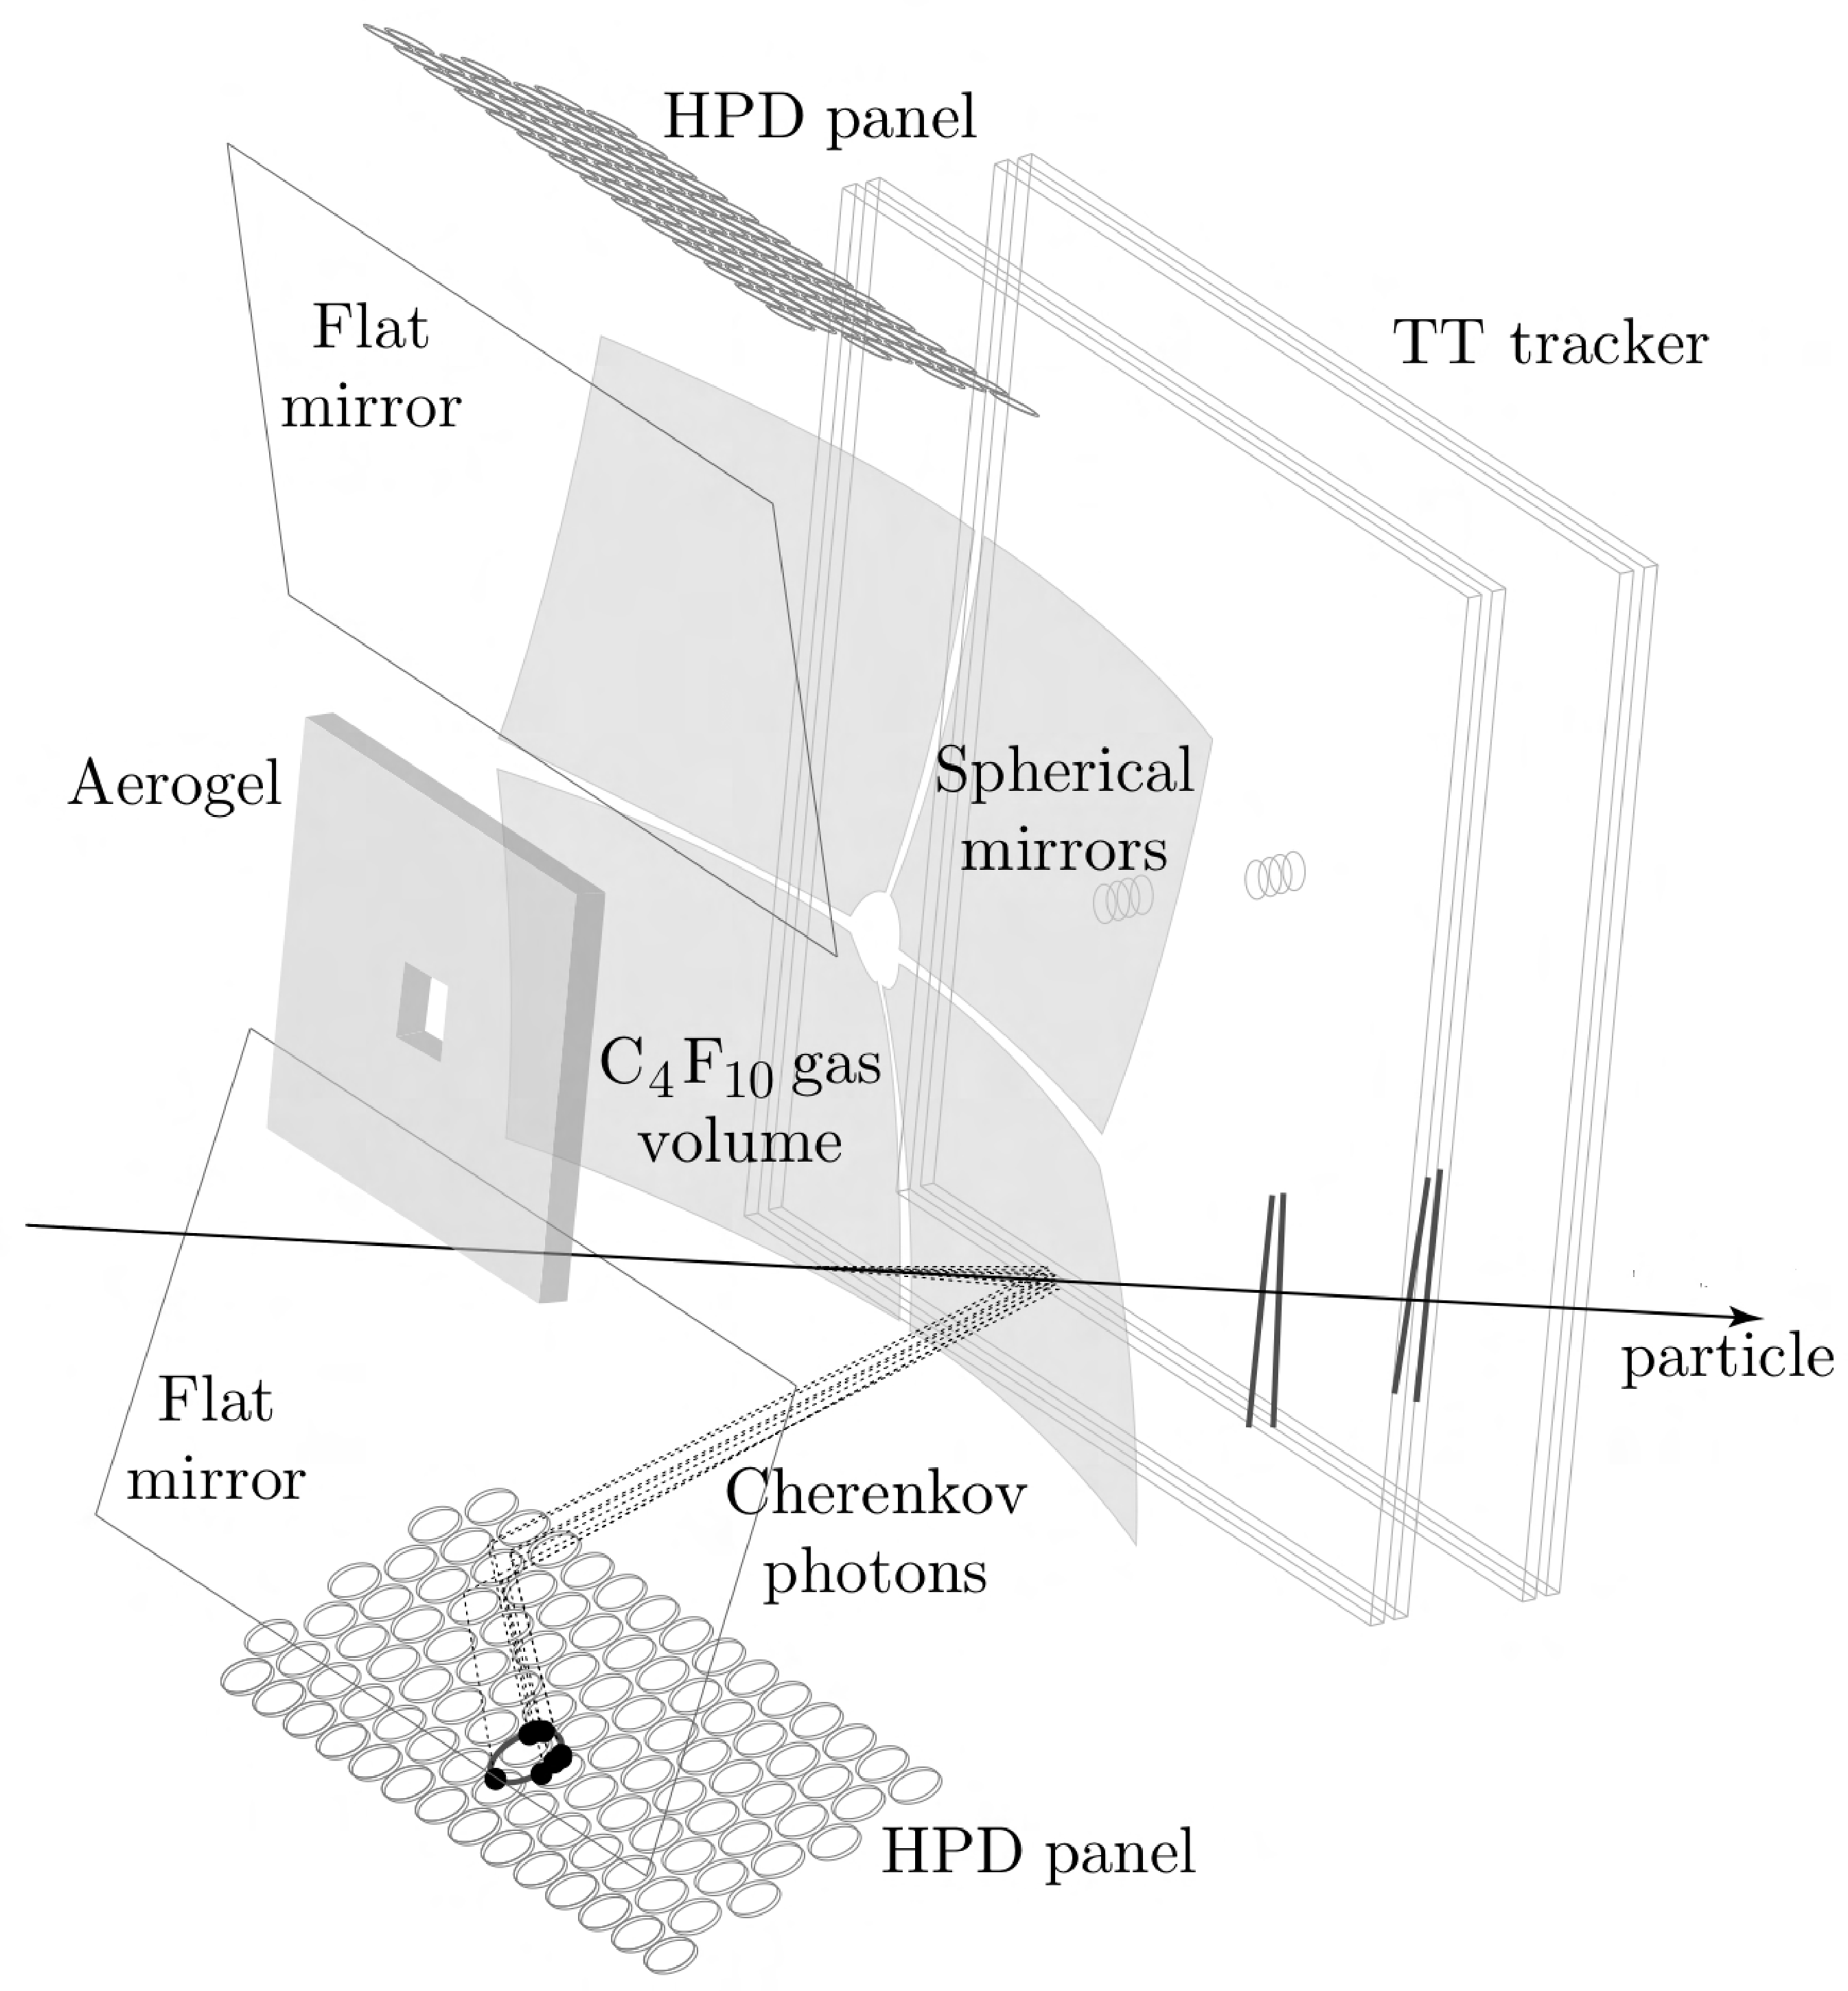
\includegraphics[width=0.48\columnwidth]{chapter3/figs/richworking.pdf}
\caption[The first \rich detector.]{An illustration of the geometry of \richone showing the path taken by Cherenkov light from the track to the photodiode~\cite{Blanks:1435718}.~\label{fig:lhcb:richgeom}}
\end{figure}
\richone provides information for particles at high polar angles
and at low momentum, from 2\gevc to 40\gevc.
It is placed before the magnet in order to limit the overall volume of gas since the detector covers the full angular 
acceptance and rotated such that the light is reflected out in the vertical plane.
The second \rich detector (\richtwo) is placed after the magnet and the downstream tracking detectors.
Both \rich detectors use the full information from the tracking system, for \richone the tracks are interpolated and for \richtwo the 
tracks are extrapolated.
\richtwo covers the high momentum region ($15 - 100 \gevc$) and the low polar angular region ($15 - 120 \mrad$) 
and the light is reflected in the horizontal plane.
Two different fluorocarbon gases are used as the Cherenkov radiators, \cfourften for \richone and \cffour for \richtwo.

The reconstruction of the Cherenkov angle for a photon ring comes from a full analytical solution 
for the \rich optics based on the mirror alignment and the position of the HPDs.
The measured Cherenkov angle can be calculated with respect to the reconstructed track position and the 
overall resolution on the Cherenkov angles for \richone and \richtwo  
is $1.618\pm0.002\mrad$ and $0.68\pm0.01\mrad$ respectively~\cite{arXiv:1211-6759}.
The Cherenkov angle for different particles from data taken in 2011 can be seen in Fig.~\ref{fig:lhcb:cherenkov}.
\begin{figure}[tbp]
\centering
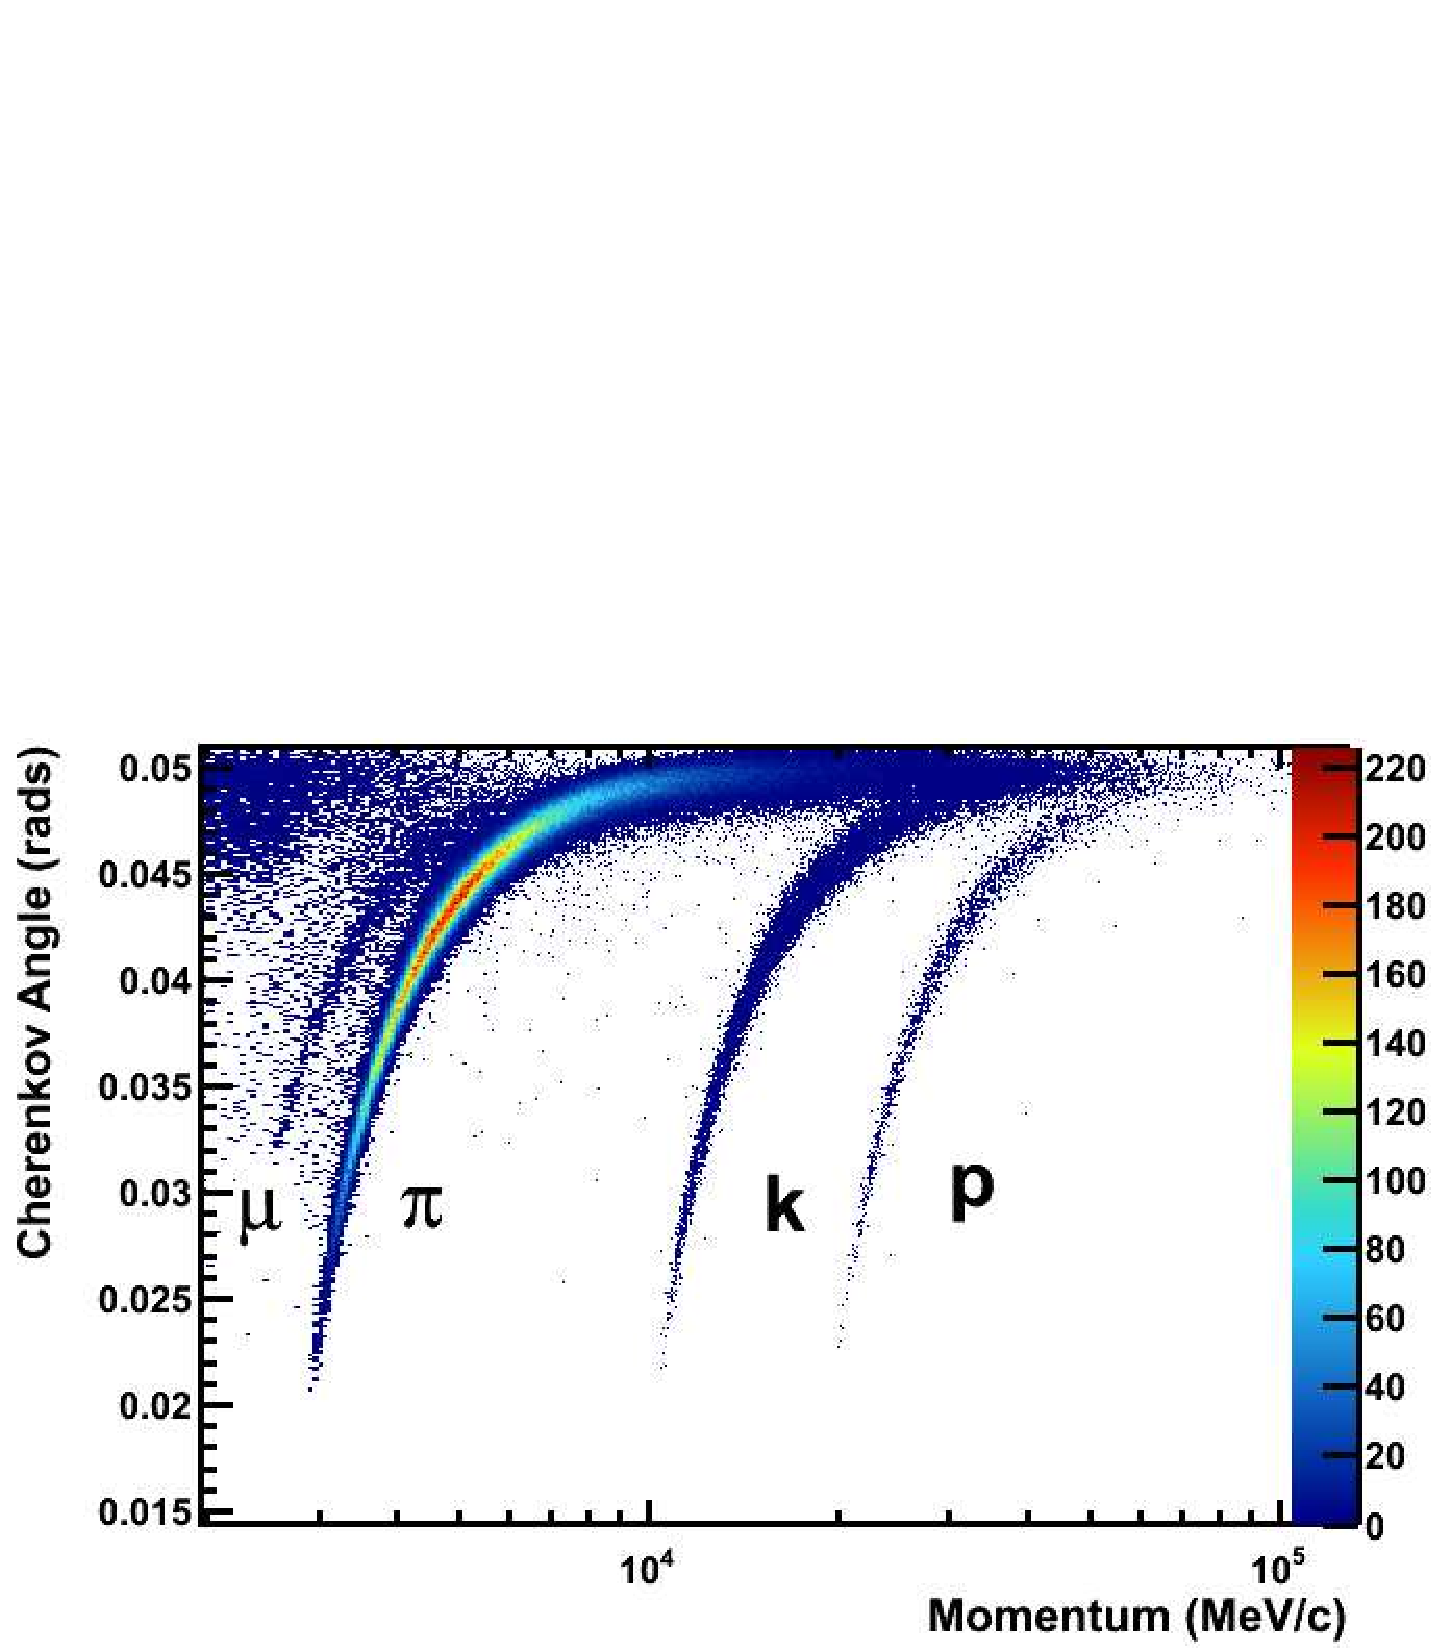
\includegraphics[width=0.48\columnwidth]{chapter3/figs/CKAnglevsMom_NoTheory_jun2011_kostas_cropped.pdf}
\caption[The Cherenkov angle for particles in the \rich detectors.]
{The Cherenkov angle for different particles as a function of momentum~\cite{arXiv:1211-6759}. 
It is possible to see the separation for kaons, pions and protons at high momenta along with the separation 
between muon and pions at low momenta.~\label{fig:lhcb:cherenkov}}
\end{figure}
The \rich detector system not only provides clear separation between kaons and pion, 
but also between muons with low momenta and high momentum protons.

The particle identification was obtained by calculating the degree to which the track matches the ring for a given mass 
when compared to the assumption that the track was a pion.
This is due to the abundance of charged pions in $pp$ collisions.
The likelihood ($\mathcal{L}$) that the Cherenkov angle came from a pion for all the tracks and rings 
is calculated for a given event. 
This calculation is changed on a track-by-track basis by testing different mass hypothesis.
The measure of particle identification is then the difference between the 
optimal calculation, i.e. the best set of mass hypotheses for all tracks in the event, 
compared to the assumption that all tracks are pions.
This results in a \dll value between all tracks in the event.
The distribution of \dllkpi for pions and kaons is given in
Fig.~\ref{fig:lhcb:dll}.
\begin{figure}[tbp]
\centering
\subfigure[]{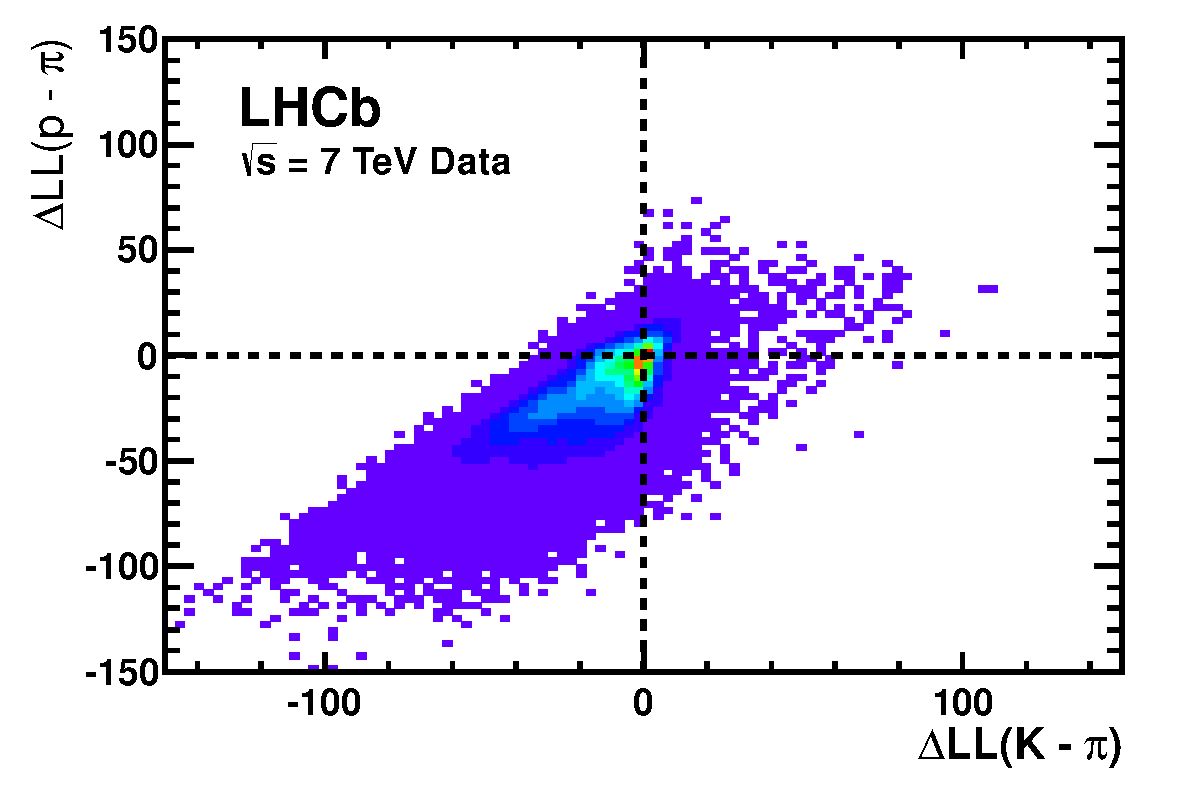
\includegraphics[width=0.48\columnwidth]{chapter3/figs/DLL2D_Pion.pdf}}
\subfigure[]{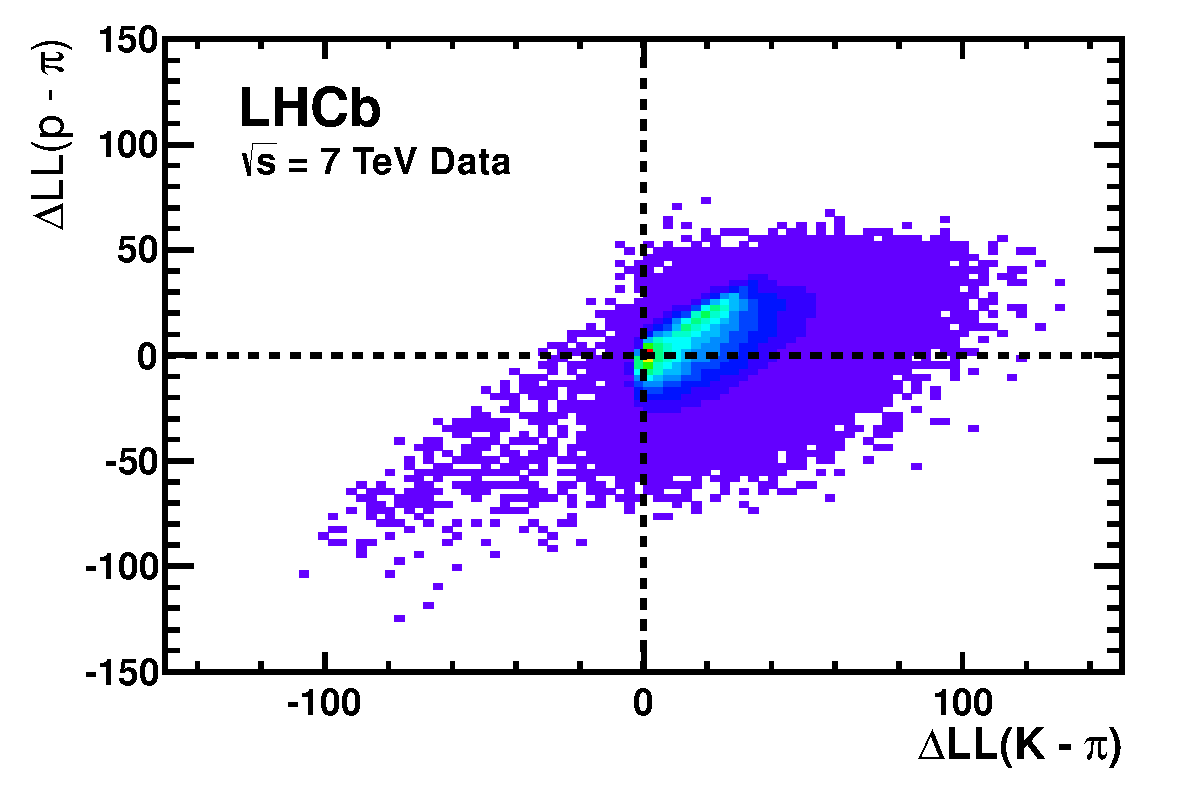
\includegraphics[width=0.48\columnwidth]{chapter3/figs/DLL2D_Kaon.pdf}}
\caption[\dllkpi distribution for kaons and pions.]
{ Distributions of (a) pions and (b) kaons showing the separation available when using the 
\dllkpi and the \dllppi variables. Separation between pions and kaons can be achieved be 
selecting tracks with a \dllkpi greater or less than zero~\cite{arXiv:1211-6759}.~\label{fig:lhcb:dll}}
\end{figure}
The resolution on the Cherenkov angle is close to what is expected from simulations of the \rich detectors
and is it possible to achieve excellent kaon and pion separation when using the \dll measures.

\subsubsection{Muon identification}

There are five muon detectors in \lhcb which are situated over 15m away from the interaction point.
The first muon station is situated before the calorimeters and 
%is used to provide \pt information for the first level hardware trigger.
the remaining four stations are the last elements of \lhcb downstream of the interaction point.
Each of the rectangular muon stations has projective geometry, meaning that the angular acceptance is equivalent for each station.
In the horizontal, bending plane, the muon stations cover from 20 to 306 \mrad and in the vertical, non-bending plane cover from 16 to 258\mrad.
Each station consists of multi-wire proportional chambers (MWPCs) interleaved with iron absorbers
except for the inner part of \Mone which is made from gas-electron multiplier (\gem) detectors.
Each chamber is filled with a mixture of Argon, \cotwo and \cffour chosen to maximise charge collection efficiency. 
The chamber size increases with distance from the beam pipe to ensure there is enough precision
in the polar region with high occupancy.
Diagrams and a detailed description of the muon detector can be in found in Ref~\cite{Alves:2008zz}.

Muon identification is provided by matching track hits in the \Mtwo-5 stations~\cite{Lanfranchi:1202759} with tracks projected from the tracking system.
This results in a Boolean decision depending on whether the muons satisfy sufficient criteria based on the track momentum. 
A further measure of muon identification is provided by a \dll variable from the muon system similar to the
\rich \dll variables. This \dllmu variable tests whether a given track is compatible with the hypothesis of 
 being a muon using clearly identified sources of muons and non-muons to build a discriminant.
Information from the muon detectors is used in the trigger to inform a decision at both the hardware and software stages.
In the hardware trigger, the presence of hits in \Mtwo and \Mthree stations are used to look for a hit in \Mone to identify a muon candidate
to trigger on.
The performance of the muon identification has been tested on both 2010~\cite{AlvesJr:1492807} and 2011 data
using the `tag-and-prob' method.
The efficiency of the Boolean muon decision (\ismuon) is shown in Fig.~\ref{fig:lhcb:muon}.
\begin{figure}
\centering
\subfigure[]{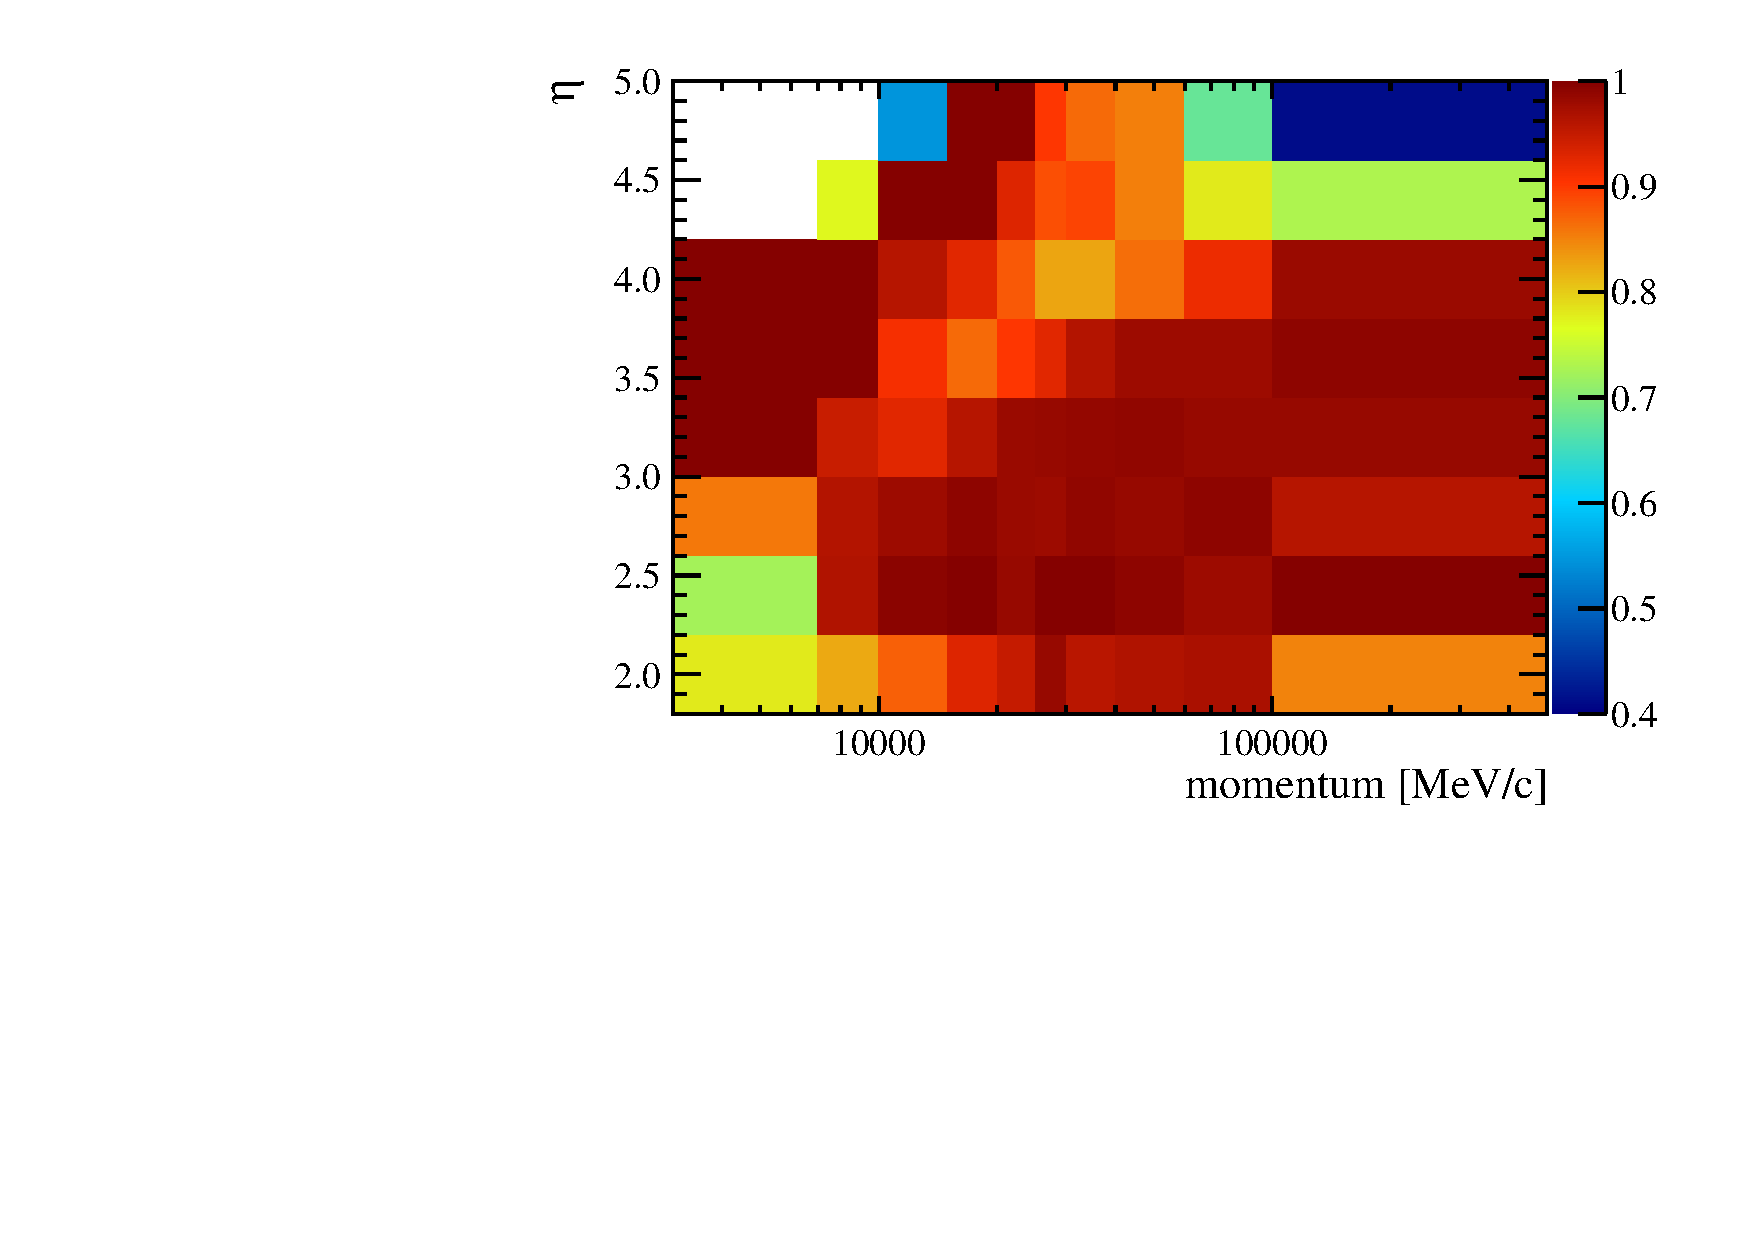
\includegraphics[width=0.48\columnwidth]{chapter3/figs/isMuonData.pdf}}
\subfigure[]{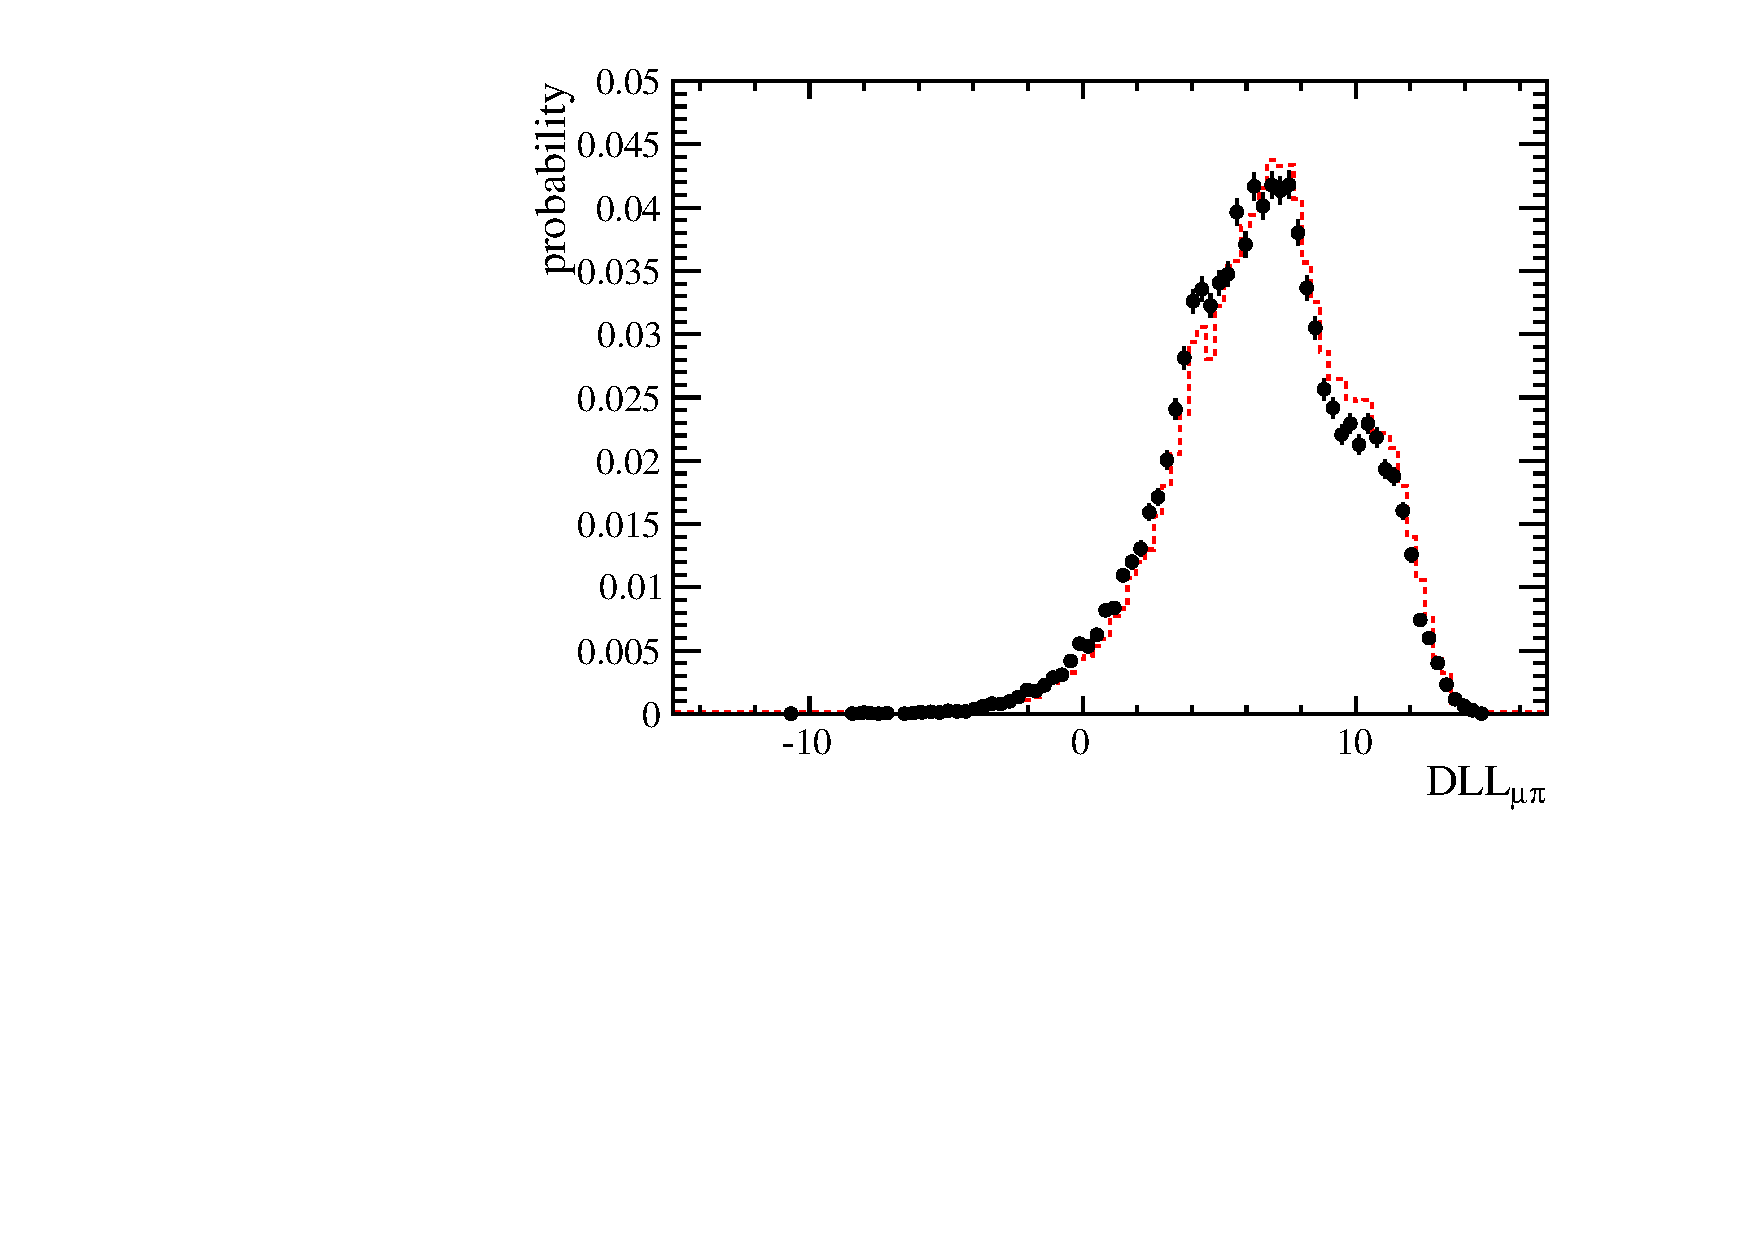
\includegraphics[width=0.48\columnwidth]{chapter3/figs/DLLmuForMuonsIsMuonFromBJpsiKHardCuts.pdf}}
\caption[The efficiency of the muon identification in \lhcb.]
{ The efficiency of the muon identification in \lhcb~\cite{MichelDeCian}.
In (a) the efficiency of the \ismuon flag as a function of muon momentum and pseudorapidity
 and in (b) the distribution of the \dllmu measure for \Bu\to\jpsi\Kp for data (points) and simulation (dotted histogram).~\label{fig:lhcb:muon} }
\end{figure}
It is possible to see that there is excellent muon identification efficiency for muons with momenta above 10\gev and 
that the \dllmu measure has excellent agreement between the data and the \lhcb simulation.



